\documentclass[a4paper,11pt]{article}
\usepackage[utf8]{inputenc}
\usepackage[T1]{fontenc}
\usepackage[french]{babel}
\usepackage{makeidx}
\usepackage{textcomp}
\usepackage{graphicx}
\usepackage{mathtools,amssymb,amsthm}
\usepackage{lmodern}
\usepackage{multirow}
\usepackage{listings}
\usepackage{array}
\usepackage{longtable}

\title{Projet de Simulation 2019 - Modèles Théoriques}
\author{Maxime Gonthier - Benjamin Guillot}

\begin{document}
\pagenumbering{gobble}\clearpage
\maketitle

\newpage
\tableofcontents

\newpage
\section{Introduction}
	Ce Rapport à pour but de présenter les trois modèles théoriques étudié pour ce projet de Simulation.\\
	Il sera composé de trois parties, chacune d'entre elles étant dédié à un modèle précis.
\section{Modèles n°1 - File M/M/N}
	\subsection{description du modèle}
	Le premier modèle est décris de la façon suivante :\\
	\textit{Le patron donne au client un ticket numéroté.\\
			Dès qu'un ordinateur se libère, la personne en attente avec le plus petit numéro de ticket accède à l'ordinateur.}
		\subsubsection{représentation}
		\centerline{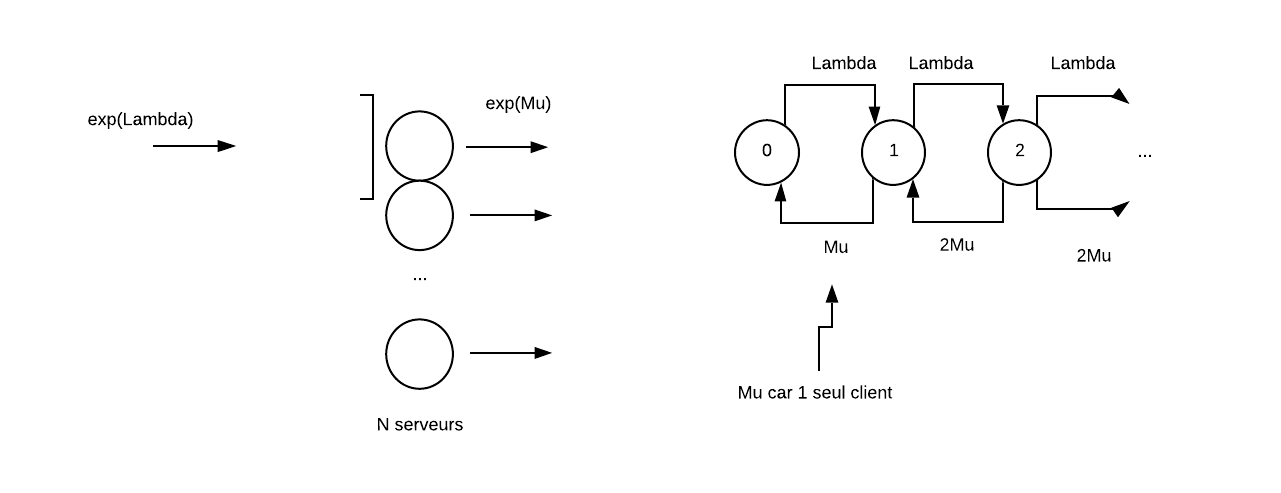
\includegraphics[scale=0.5]{MMN.png}}
		Modélisation graphique de la file M/M/N.\\
		Dans l'état i il y à i clients dans la file.\\
		L'espace d'état est défini par $E=\pmb{\mathbb{N}}$\\
		Les transitions peuvent s'exprimer de la façon suivante :\\
		$\forall i \ge 0,$\\
		$i^{\lambda} \to i + 1 $\\
		$i^{\mu} \to i - 1$\\
		\\
		La condition de convergence pour ce modèle est :\\
		$\rho > 1$
	\subsection{Données et Formules}
	On à besoin pour ce modèles de définir certaines données :\\
	$\lambda$ : probabilité d'arrivée de client.\\
	$\mu$ : le temps de service.\\
	$\rho$ : l'intensité du trafic.\\
	$N$ : le nombre de serveur, fixé à 10.\\
	\\
	On calcule l'intensité du trafic de la façon suivante pour chaque 	$\lambda$ : \\
	$\rho = \frac{\lambda}{N*\mu}$\\
	\\
	On à également besoin du nombre moyen de client théorique $Nmoyen$:\\
	$Nmoyen = E[nq(???)] = \frac{\rho * \varrho}{1-\rho}$\\
	ou $\varrho = Proba???(\ge N) = \frac{(N*\rho)^{N}}{N!(1-\rho)^{\rho_{0}}}$.\\
	\\
	Ici, $\rho_{0}$ représente la probabilité que la file soit vide et se calcule de la façon suivante :\\
	$\rho_{0} = 1 + (\frac{(N*\rho)^{N}}{N!(1-\rho)}+\sum^{N-1}_{n = 1}\frac{(N*\rho)^{N}}{n!})$\\
		\subsubsection{Temps moyen d'attente et 90 percentile}
		Maintenant que l'on a toute ces données, on peut écrire une formule pour le temps moyen d'attente de ce modèle :\\
		$E[A] = \frac{E[n_{q}]}{\lambda} = \frac{\varrho}{N*\mu(1-\rho)}$\\
		\\
		On peut donc écrire une formule pour calculer de 90 percentile du temps d'attente de ce modèle :\\
		$t_{90}[A] = \frac{E[A]}{\varrho}*ln(10\varrho)$\\
	

\section{Modèle n°2 - File M/M/1}
	\subsection{description du modèle}
	Le second modèle est décris de la façon suivante :\\
	\textit{Le patron choisit au hasard, uniformément un ordinateur parmis les N puis il donne au client un ticket numéroté pour l'ordinateur choisi.\\
			Dès que le client d'un ordinateur a fini, c'est le client qui a le plus petit numéro parmis ceux affecté à cet ordinateur qui prend la place.}
	\subsubsection{représentation}
	\centerline{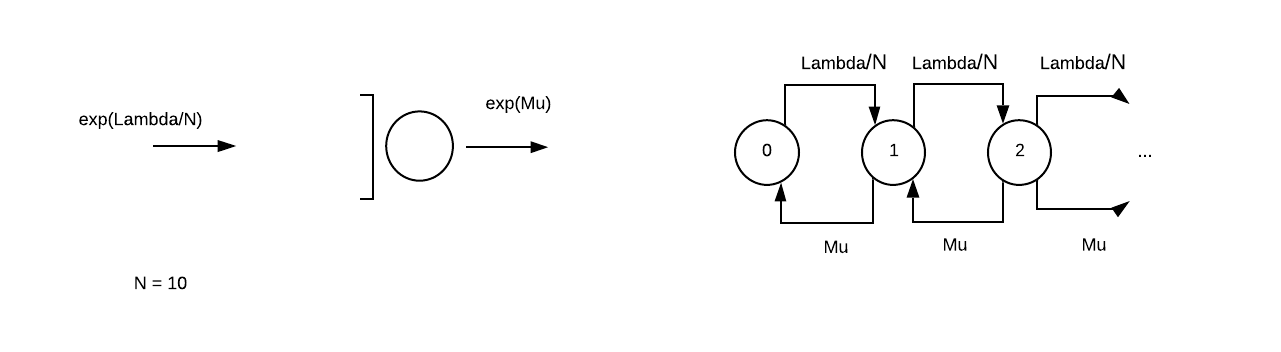
\includegraphics[scale=0.5]{MM1.png}}
	Modélisation graphique de la file M/M/1.\\
	Les transitions peuvent s'exprimer de la façon suivante :\\
		\begin{tabular}{ | c | c | c | c |}
		\hline
		\ & 0          & 1                 & 2\\			
		0 & $-\lambda$ & $\lambda$         & 0\\
		1 & $\mu$      & $-(\lambda + \mu)$& $\lambda$\\
		2 & 0          & $\mu$             &  $-(\lambda + \mu)$\\
		\hline  
		\end{tabular}\\
		$\forall i \epsilon \pmb{\mathbb{N}},$\\
		$Q_{i, i+1} = \lambda$\\
		$Q_{i, i-1} = \mu$\\
		La condition de convergence pour ce modèle est :\\
		$\rho < 1$
	\subsection{Données et Formules}
	Pour ce modèles, on utilise les même données que pour le modèles précédent soit :\\
	$\lambda$ : probabilité d'arrivée de client.\\
	$\mu$ : le temps de service.\\
	$\rho$ : l'intensité du trafic.\\
	\\
	Cependant on calcule $\rho$ différemment :\\
	$\rho = \frac{\lambda}{\mu}$\\
	\\
	Le nombre moyen de client s'exprime ainsi:\\
	$Nmoyen = \frac{\rho}{1-\rho}$
		\subsubsection{Temps moyen d'attente et 90 percentile}
		Le temps d'attente moyen est :\\
		$E[A] = \rho * \frac{\frac{1}{\mu}}{1-\rho}$
		\\
		Le 90 percentile du temps d'attente s'exprime donc de la façon suivante :\\
		$max(0,\frac{E[A]}{\rho}ln(10*\rho))$
\end{document}
